% **************************************************************************************************************
% A Classic Thesis Style
% An Homage to The Elements of Typographic Style
%
% Copyright (C) 2010 Andr� Miede http://www.miede.de
%
% If you like the style then I would appreciate a postcard. My address 
% can be found in the file ClassicThesis.pdf. A collection of the 
% postcards I received so far is available online at 
% http://postcards.miede.de
%
% License:
% This program is free software; you can redistribute it and/or modify
% it under the terms of the GNU General Public License as published by
% the Free Software Foundation; either version 2 of the License, or
% (at your option) any later version.
%
% This program is distributed in the hope that it will be useful,
% but WITHOUT ANY WARRANTY; without even the implied warranty of
% MERCHANTABILITY or FITNESS FOR A PARTICULAR PURPOSE.  See the
% GNU General Public License for more details.
%
% You should have received a copy of the GNU General Public License
% along with this program; see the file COPYING.  If not, write to
% the Free Software Foundation, Inc., 59 Temple Place - Suite 330,
% Boston, MA 02111-1307, USA.
%
% **************************************************************************************************************
% Note:
%    * You must not use "u etc. in strings/commands that will be spaced out (use \"u or real umlauts instead)
%    * New enumeration (small caps): \begin{aenumerate} \end{aenumerate}
%    * For margin notes: \graffito{}
%    * Do not use bold fonts in this style, it is designed around them
%    * Use tables as in the examples
%    * See classicthesis-ldpkg.sty for useful commands
% **************************************************************************************************************
% To Do:
%		 * [high] Check this out: http://www.golatex.de/koma-script-warnung-in-verbindung-mit-listings-package-t2058.html
%    * [medium] mathbb in section-titles/chapter-titles => disappears somehow in headlines!!!
%    * [low] Calculate text block size for Libertine font
%    * [low] Think about processing a4paper, a5paper, 10pt, 11pt, 12pt etc. options for typearea layout
%            (store values in internal variables and handle by \AtEndOfPackage{\areaset...})
% **************************************************************************************************************
\documentclass[ oneside,openright,titlepage,fleqn,numbers=noenddot,headinclude,%1headlines,% 
                11pt,a4paper,BCOR5mm,footinclude,cleardoublepage=empty,abstractoff,dottedtoc % <--- obsolete, remove (todo)
                ]{scrreprt}

% ********************************************************************
% Development Stuff
% ********************************************************************
\listfiles
%\usepackage[l2tabu, orthodox, abort]{nag}
%\usepackage[warning, all]{onlyamsmath}
% ********************************************************************
% Re-usable information
% ********************************************************************
\newcommand{\myTitle}{A Classic Thesis Style\xspace}
\newcommand{\myDegree}{An Homage to The Elements of Typographic Style\xspace}
\newcommand{\myName}{Andr\'e Miede\xspace}
\newcommand{\myProf}{Put name here\xspace}
\newcommand{\myOtherProf}{Put name here\xspace}
\newcommand{\mySupervisor}{Put name here\xspace}
\newcommand{\myFaculty}{Put data here\xspace}
\newcommand{\myDepartment}{Put data here\xspace}
\newcommand{\myUni}{\protect{Put data here}\xspace}
\newcommand{\myLocation}{Darmstadt\xspace}
\newcommand{\myTime}{May 2010\xspace}
\newcommand{\myVersion}{Version 2.8\xspace}
%*******************************************************
% Packages with options that might require adjustments
%*******************************************************
\usepackage[latin1]{inputenc} 
\usepackage[ngerman,american]{babel}           
% Maxnames gibt an wie viele Autoren ausgeschrieben werden.
% BibliographyStrings setzt den zu verwendenten Verkuerzungsstrings bei ueberschreiten (hier: et al.)
\usepackage[natbib=true,style=authoryear,maxnames=2]{biblatex}
\DefineBibliographyStrings{ngerman}{andothers={et \addabbrvspace al\adddot}}

% TODO: Pfad zur BibLaTeX Datei anpassen.
\bibliography{Bibliography}
\usepackage[fleqn]{amsmath} % math environments and more by the AMS 

%*******************************************************
\usepackage{classicthesis-ldpkg} % [backref]
%*******************************************************
% Options for classicthesis.sty:
% tocaligned eulerchapternumbers drafting linedheaders listsseparated 
% subfig nochapters beramono eulermath parts minionpro pdfspacing 
% listings dottedtoc minionprospacing manychapters
\usepackage[eulerchapternumbers,drafting,listings,listsseparated,%pdfspacing,%listings,
						subfig,beramono,eulermath,parts]{classicthesis}

%*******************************************************
% Some font experiments
%*******************************************************
%\usepackage[osf]{libertine}
%\usepackage{hfoldsty}
%\usepackage[light,condensed,math]{iwona}
%\renewcommand{\sfdefault}{iwona}
%\usepackage{lmodern} % <-- no osf support :-(
%\usepackage[urw-garamond]{mathdesign} <-- no osf support :-(

%*******************************************************
% Fine-tuning for the text area
%*******************************************************
%\linespread{1.05} % a bit more for Palatino
%\areaset[5mm]{312pt}{761pt} % 686 (factor 2.2) + 33 head + 42 head \the\footskip
%\setlength{\marginparwidth}{7em}%
%\setlength{\marginparsep}{2em}%

%*******************************************************
% hack to use citations in float environments 
% will be fixed with caption package version 3.2
%*******************************************************
\usepackage{makerobust} 
\makeatletter 
\MakeRobustCommand\caption@xref 
\makeatother 

%*******************************************************            
%\usepackage[section,below]{placeins} <--- not everybody wants this
%\usepackage[all]{hypcap} <--- does not work with MiKTeX 2.6
% ********************************************************************
% Language/strings for backrefs (change here, thanks, Lorenzo)
%*******************************************************
%\renewcommand{\backrefnotcitedstring}{\relax}%(Not cited.)
%\renewcommand{\backrefcitedsinglestring}[1]{(Citato a pagina~#1.)}
%\renewcommand{\backrefcitedmultistring}[1]{(Citato alle pagine~#1.)}
%\renewcommand{\backreftwosep}{ e~}
%\renewcommand{\backreflastsep}{ e~}
% ********************************************************************
% Setup and Finetuning
%*******************************************************
\newlength{\abcd} % for ab..z string length calculation
\newcommand{\myfloatalign}{\centering} % how all the floats will be aligned
\setlength{\extrarowheight}{3pt} % increase table row height
% ********************************************************************
% Captions look and feel
%*******************************************************
\captionsetup{format=hang,font=small}
% ********************************************************************
% Listings setup
% ********************************************************************
%\lstset{emph={trueIndex,root},emphstyle=\color{BlueViolet}}%\underbar} % for special keywords
% ********************************************************************
\lstset{%C++,
    keywordstyle=\color{RoyalBlue},%\bfseries,
    basicstyle=\small\ttfamily,
    %identifierstyle=\color{NavyBlue},
    commentstyle=\color{Green}\ttfamily,
    stringstyle=\rmfamily,
    numbers=none,%left,%
    numberstyle=\scriptsize,%\tiny
    stepnumber=5,
    numbersep=8pt,
    showstringspaces=false,
    breaklines=true,
    frameround=ftff,
    frame=single,
    belowcaptionskip=.75\baselineskip,
    numberbychapter=false
    %frame=L
} 

% ********************************************************************
% Where to look for graphics
%*******************************************************
%\graphicspath{{gfx/}{misc/}} % considered harmful according to l2tabu
% ********************************************************************
% Hyperreferences
%*******************************************************
\hypersetup{%
    colorlinks=true, linktocpage=true, pdfstartpage=3, pdfstartview=FitV,%
    % uncomment the following line if you want to have black links (e.g., for printing)
    %colorlinks=false, linktocpage=false, pdfborder={0 0 0}, pdfstartpage=3, pdfstartview=FitV,% 
    breaklinks=true, pdfpagemode=UseNone, pageanchor=true, pdfpagemode=UseOutlines,%
    plainpages=false, bookmarksnumbered, bookmarksopen=true, bookmarksopenlevel=1,%
    hypertexnames=true, pdfhighlight=/O,%hyperfootnotes=true,%nesting=true,%frenchlinks,%
    urlcolor=webbrown, linkcolor=RoyalBlue, citecolor=webgreen, %pagecolor=RoyalBlue,%
    %urlcolor=Black, linkcolor=Black, citecolor=Black, %pagecolor=Black,%
    pdftitle={\myTitle},%
    pdfauthor={\textcopyright\ \myName, \myUni, \myFaculty},%
    pdfsubject={},%
    pdfkeywords={},%
    pdfcreator={pdfLaTeX},%
    pdfproducer={LaTeX with hyperref and classicthesis}%
}

%********************************************************************
% Hyphenation
%*******************************************************
%\hyphenation{put special hyphenation here}
% ********************************************************************
% GO!GO!GO! MOVE IT!
%*******************************************************
\begin{document}
\frenchspacing
\raggedbottom
\selectlanguage{american} % american ngerman
%\renewcommand*{\bibname}{new name}
%\setbibpreamble{}
\pagenumbering{roman}
\pagestyle{plain}
%********************************************************************
% Frontmatter
%*******************************************************
%*******************************************************
% Little Dirty Titlepage
%*******************************************************
\thispagestyle{empty}
%\pdfbookmark[1]{Titel}{title}
%*******************************************************
\begin{center}
    \spacedlowsmallcaps{\myName} \\ \medskip                        

    \begingroup
        \color{Maroon}\spacedallcaps{\myTitle}
    \endgroup
\end{center}        

%*******************************************************
% Titlepage
%*******************************************************
\begin{titlepage}
	% if you want the titlepage to be centered, uncomment and fine-tune the line below (KOMA classes environment)
	\begin{addmargin}[-1cm]{-3cm}
    \begin{center}
        \large  

        \hfill

        \vfill

        \begingroup
            \color{Maroon}\spacedallcaps{\myTitle} \\ \bigskip
        \endgroup

        \spacedlowsmallcaps{\myName} \\
        
        \spacedlowsmallcaps{\myPersonId}

        \vfill

        % 
\includegraphics[width=6cm]{gfx/TFZsuperellipse_bw} \\ \medskip

        %\myDegree \\ \medskip   
        %\myDepartment \\                            
        \myFaculty \\
        \myUni \\ \bigskip

        \myTime

        \vfill                      

    \end{center}  
  \end{addmargin}       
\end{titlepage}   
\thispagestyle{empty}

\hfill

\vfill

\noindent\myName: \textit{\myTitle,} \myDegree, \textcopyright\ \myTime

%\bigskip
%
%\noindent\spacedlowsmallcaps{Supervisors}: \\
%\myProf \\
%\myOtherProf \\ 
%\mySupervisor
%
%\medskip
%
%\noindent\spacedlowsmallcaps{Location}: \\
%\myLocation
%
%\medskip
%
%\noindent\spacedlowsmallcaps{Time Frame}: \\
%\myTime

\cleardoublepage%*******************************************************
% Dedication
%*******************************************************
\thispagestyle{empty}
%\phantomsection 
\refstepcounter{dummy}
\pdfbookmark[1]{Dedication}{Dedication}

\vspace*{3cm}

\begin{center}
    \emph{Ohana} means family. \\
    Family means nobody gets left behind, or forgotten. \\ \medskip
    --- Lilo \& Stitch    
\end{center}

\medskip

\begin{center}
    Dedicated to the loving memory of Rudolf Miede. \\ \smallskip
    1939\,--\,2005
\end{center}
\cleardoublepage%*******************************************************
% Abstract
%*******************************************************
%\renewcommand{\abstractname}{Abstract}
\pdfbookmark[1]{Abstract}{Abstract}
\begingroup
\let\clearpage\relax
\let\cleardoublepage\relax
\let\cleardoublepage\relax

\chapter*{Abstract}
Short summary of the contents in English\dots

\endgroup			

\vfill
\cleardoublepage%*******************************************************
% Publications
%*******************************************************
\pdfbookmark[1]{Publications}{publications}
\chapter*{Publications}
Some ideas and figures have appeared previously in the following publications:

\bigskip

\noindent Put your publications from the thesis here.
\cleardoublepage%*******************************************************
% Acknowledgments
%*******************************************************
\pdfbookmark[1]{Acknowledgments}{acknowledgments}

\begin{flushright}{\slshape    
    We have seen that computer programming is an art, \\ 
    because it applies accumulated knowledge to the world, \\ 
    because it requires skill and ingenuity, and especially \\
    because it produces objects of beauty.} \\ \medskip
    --- \defcitealias{knuth:1974}{Donald E. Knuth}\citetalias{knuth:1974} \citep{knuth:1974}
\end{flushright}



\bigskip

\begingroup
\let\clearpage\relax
\let\cleardoublepage\relax
\let\cleardoublepage\relax
\chapter*{Acknowledgments}
Put your acknowledgments here.

Many thanks to everybody who already sent me a postcard!

Regarding the typography and other help, many thanks go to Marco 
Kuhlmann, Philipp Lehman, Lothar Schlesier, Jim Young, Lorenzo 
Pantieri and Enrico Gregorio\footnote{Members of GuIT (Gruppo 
Italiano Utilizzatori di \TeX\ e \LaTeX )}, J\"org Sommer, 
Joachim K\"ostler, Daniel Gottschlag, Denis Aydin, Paride 
Legovini, Steffen Prochnow, Nicolas Repp, Hinrich Harms, 
and the whole \LaTeX-community for support, ideas and some great software.

\endgroup




\pagestyle{scrheadings}
\cleardoublepage%*******************************************************
% Table of Contents
%*******************************************************
%\phantomsection
\refstepcounter{dummy}
\pdfbookmark[1]{\contentsname}{tableofcontents}
\setcounter{tocdepth}{2} % <-- 2 includes up to subsections in the ToC
\setcounter{secnumdepth}{3} % <-- 3 numbers up to subsubsections
\manualmark
\markboth{\spacedlowsmallcaps{\contentsname}}{\spacedlowsmallcaps{\contentsname}}
\tableofcontents 
\automark[section]{chapter}
\renewcommand{\chaptermark}[1]{\markboth{\spacedlowsmallcaps{#1}}{\spacedlowsmallcaps{#1}}}
\renewcommand{\sectionmark}[1]{\markright{\thesection\enspace\spacedlowsmallcaps{#1}}}%*******************************************************
% List of Figures and of the Tables
%*******************************************************
\clearpage

\begingroup 
    \let\clearpage\relax
    \let\cleardoublepage\relax
    \let\cleardoublepage\relax
    %*******************************************************
    % List of Figures
    %*******************************************************    
    %\phantomsection 
    \refstepcounter{dummy}
    %\addcontentsline{toc}{chapter}{\listfigurename}
    \pdfbookmark[1]{\listfigurename}{lof}
    \listoffigures

    \vspace*{8ex}

    %*******************************************************
    % List of Tables
    %*******************************************************
    %\phantomsection 
    \refstepcounter{dummy}
    %\addcontentsline{toc}{chapter}{\listtablename}
    \pdfbookmark[1]{\listtablename}{lot}
    \listoftables
        
    \vspace*{8ex}
%   \newpage
    
    %*******************************************************
    % List of Listings
    %*******************************************************      
	  %\phantomsection 
    \refstepcounter{dummy}
    %\addcontentsline{toc}{chapter}{\lstlistlistingname}
    \pdfbookmark[1]{\lstlistlistingname}{lol}
    \lstlistoflistings 

    \vspace*{8ex}
       
    %*******************************************************
    % Acronyms
    %*******************************************************
    %\phantomsection 
    \refstepcounter{dummy}
    \pdfbookmark[1]{Acronyms}{acronyms}
    \markboth{\spacedlowsmallcaps{Acronyms}}{\spacedlowsmallcaps{Acronyms}}
    \chapter*{Acronyms}
    \begin{acronym}
        \acro{GUI}{graphical user interface}
    \end{acronym}                     
\endgroup

\cleardoublepage
%********************************************************************
% Mainmatter
%*******************************************************
\pagenumbering{arabic}
% use \cleardoublepage here to avoid problems with pdfbookmark
\cleardoublepage\part{Some Kind of Manual}
%************************************************
\chapter{Introduction}\label{ch:introduction}
%************************************************

This report shall provide detailed information about the implementation of the cabin manager application.

\subsection{Attributes}
\label{subsec:attributes}

Apart from the mandatory attributes, the following attributes were chosen to be implemented as well:
\begin{description}
\item[Size:] The area of available space in the cabin.
\item[Condition:] The condition the cabin is in. Only the following values are allowed: \texttt{PERFECT}, \texttt{GOOD}, \texttt{FAIR}, \texttt{BAD}, \texttt{IN\_SHAMBLES}, \texttt{UNKNOWN}. The limitation to these attributes is achieved by utilizing an \texttt{enumeration}.
\end{description}

\subsection{Cost calculation}
\label{subsec:cost_calculation}

The calculation of a cabin's cost for one night, are calculated according to the following formula:

\texttt{BASIC\_COST + CONDITION\_COST + FACILITIES\_COST + SIZE\_COST + (BED\_TO\_ROOM\_RATIO * BED\_TO\_ROOM\_MULTIPLIER)}

\texttt{BASIC\_COST} and \texttt{BED\_TO\_ROOM\_MULTIPLIER} are constants that can be set in the \texttt{cabin} class.
\cleardoublepage\part{The Showcase}
%*****************************************
\chapter{UML exercise one}\label{ch:uml}
%*****************************************

From the textual description of the use case the following use case diagram was derived:

\begin{figure}[H]
\begin{centering}
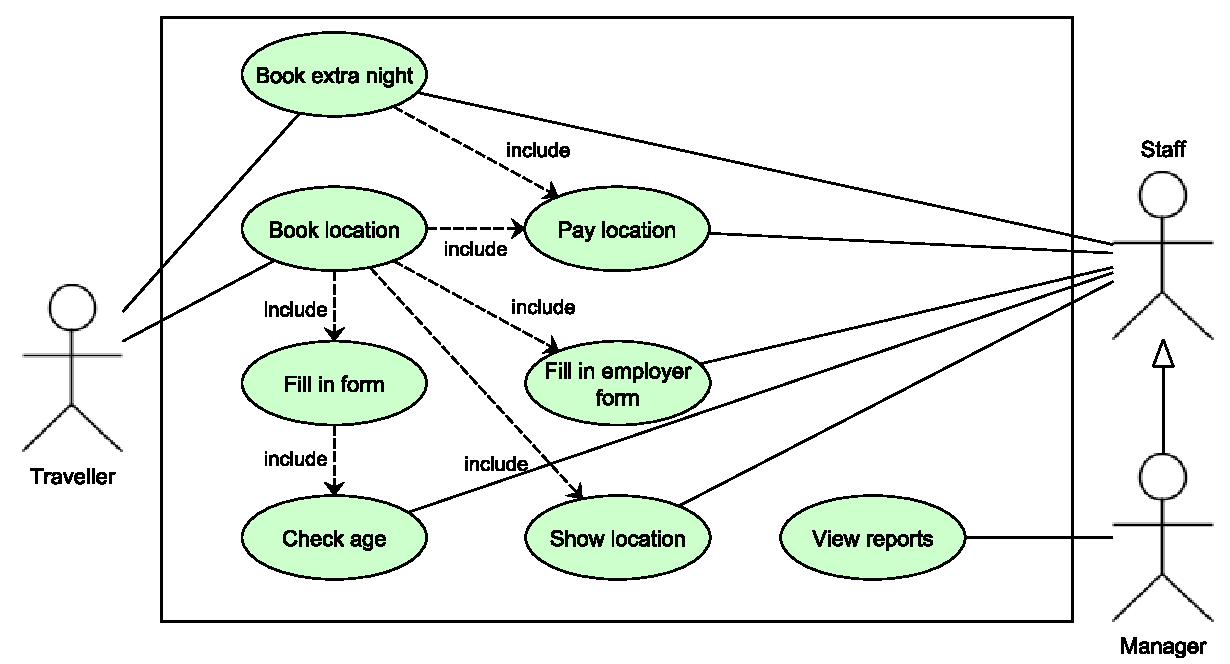
\includegraphics[width=\textwidth]{gfx/usecase.pdf} 
\end{centering}
\caption{Use case diagram.}
\label{fig:usecase}
\end{figure}

The complexity level with many \textit{include} cases was choose to justify the use of a diagram and to show the possible sub-cases that might be reused.

Following from this description the \textit{book location} high-ceremony use case would look like the following scenario:

\section{High ceremony use cases}

\subsection{Use case: book location}

\begin{description}
\item[Goal:] Book a location.
\item[Actors:] Traveller, Staff.
\item[Precondition:] A location is available.
\item[Postcondition:] The traveller has booked a location for one night.
\item[Steps:]
\begin{enumerate}
\item Traveller \textit{fills in form}.
\item Staff \textit{fills in employer form}.
\item Traveller \textit{pays location}.
\item Staff \textit{shows location} to traveller.
\end{enumerate}

\item[Alternatives:]
\begin{enumerate}
\item[1A.] Fill in form use case fails.\\
The booking fails.
\item[3A.] Pay location use case fails.\\
The booking fails.
\end{enumerate}
\end{description}

\subsection{Use case: fill in form}

\begin{description}
\item[Goal:] Fill in form.
\item[Actors:] Traveller, Staff.
\item[Precondition:] User wants to book a location.
\item[Postcondition:] Form was filled in correct.
\item[Steps:]
\begin{enumerate}
\item Traveller enters personal details.
\item Traveller provides staff with passport.
\item Staff \textit{checks age}.
\item Staff returns passport.
\end{enumerate}

\item[Alternatives:]
\begin{enumerate}
\item[3A.] Check age use case fails.\\
The booking fails.
\end{enumerate}
\end{description}

\subsection{Use case: pay location}

\begin{description}
\item[Goal:] Pay for stay.
\item[Actors:] Traveller, Staff.
\item[Precondition:] -
\item[Postcondition:] -
\item[Steps:] 
\begin{enumerate}
\item Traveller pays for one night.
\item Staff accepts payment.
\item Staff marks payment as received.
\end{enumerate}

\item[Alternatives:]
\begin{enumerate}
\item[1A.] Traveller can not pay for stay.\\
The payment fails.
\end{enumerate}
\end{description}

\subsection{Use case: show location}

\begin{description}
\item[Goal:] Traveller is shown location.
\item[Actors:] Traveller, Staff.
\item[Precondition:] -
\item[Postcondition:] -
\item[Steps:] 
\begin{enumerate}
\item Staff shows traveller the location.
\end{enumerate}

\item[Alternatives:] -
\end{description}

\subsection{Use case: fill in employee form}

\begin{description}
\item[Goal:] Employee fills in form.
\item[Actors:] Staff.
\item[Precondition:] -
\item[Postcondition:] -
\item[Steps:] 
\begin{enumerate}
\item Staff enter details (location id, form number, nights to stay).
\end{enumerate}

\item[Alternatives:] -
\end{description}

\section{Activity diagrams}

\subsection{Book location}

\begin{figure}[H]
\begin{centering}
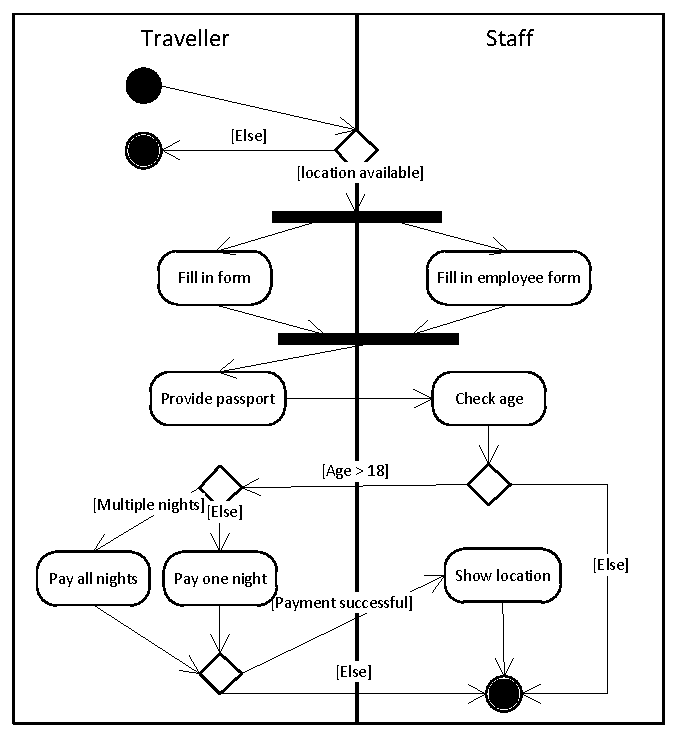
\includegraphics[width=\textwidth]{gfx/activity_diagram_book.pdf} 
\end{centering}
\caption{Activity diagram of book location.}
\label{fig:actdiag_book}
\end{figure}

Even though best practice is to only have one end-point per activity diagram, the provided activity diagram has two to improve readability.

\subsection{GetCost()}


%\addtocontents{toc}{\protect\clearpage} % <--- just debug stuff, ignore
%************************************************
\chapter{Source Code}\label{ch:source_code} % $\mathbb{ZNR}$
%************************************************

%*****************************************

%\include{multiToC} % <--- just debug stuff, ignore for your documents
% ********************************************************************
% Backmatter
%*******************************************************
\appendix
\cleardoublepage\part{Appendix}
%********************************************************************
% Appendix
%*******************************************************
\chapter{Appendix Test}

%********************************************************************
% Other Stuff in the Back
%*******************************************************
\cleardoublepage%********************************************************************
% Bibliography
%*******************************************************
% work-around to have small caps also here in the headline
\manualmark
\markboth{\spacedlowsmallcaps{\bibname}}{\spacedlowsmallcaps{\bibname}} % work-around to have small caps also
%\phantomsection 
\refstepcounter{dummy}
\addtocontents{toc}{\protect\vspace{\beforebibskip}} % to have the bib a bit from the rest in the toc
\addcontentsline{toc}{chapter}{\tocEntry{\bibname}}
\printbibliography{}
\label{app:bibliography} 
\cleardoublepage\pagestyle{empty}

\hfill

\vfill


\pdfbookmark[0]{Colophon}{colophon}
\section*{Colophon}
This thesis was typeset with \LaTeXe\ using Hermann Zapf's
\emph{Palatino}
and \emph{Euler} type faces (Type~1 PostScript fonts \emph{URW
Palladio L}
and \emph{FPL} were used). The listings are typeset in \emph{Bera
Mono}, originally developed by Bitstream, Inc. as ``Bitstream Vera''.
(Type~1 PostScript fonts were made available by Malte Rosenau and
Ulrich Dirr.)

The typographic style was inspired by \cauthor{bringhurst:2002}'s genius as
presented in \emph{The Elements of Typographic Style} 
\citep{bringhurst:2002}. It is available for \LaTeX\ via \textsmaller{CTAN} as 
``\href{http://www.ctan.org/tex-archive/macros/latex/contrib/classicthesis/}%
{\texttt{classicthesis}}''.

\paragraph{note:} The custom size of the textblock was calculated
using the directions given by Mr. Bringhurst (pages 26--29 and
175/176). 10~pt Palatino needs  133.21~pt for the string
``abcdefghijklmnopqrstuvwxyz''. This yields a good line length between
24--26~pc (288--312~pt). Using a ``\emph{double square textblock}''
with a 1:2 ratio this results in a textblock of 312:624~pt (which
includes the headline in this design). A good alternative would be the
``\emph{golden section textblock}'' with a ratio of 1:1.62, here
312:505.44~pt. For comparison, \texttt{DIV9} of the \texttt{typearea}
package results in a line length of 389~pt (32.4~pc), which is by far
too long. However, this information will only be of interest for
hardcore pseudo-typographers like me.%

To make your own calculations, use the following commands and look up
the corresponding lengths in the book:
\begin{verbatim}
    \settowidth{\abcd}{abcdefghijklmnopqrstuvwxyz}
    \the\abcd\ % prints the value of the length
\end{verbatim}
Please see the file \texttt{classicthesis.sty} for some precalculated 
values for Palatino and Minion.

    \settowidth{\abcd}{abcdefghijklmnopqrstuvwxyz}
    \the\abcd\ % prints the value of the length


\bigskip

\noindent\finalVersionString




\cleardoublepage%*******************************************************
% Declaration
%*******************************************************
\refstepcounter{dummy}
\pdfbookmark[0]{Declaration}{declaration}
\chapter*{Declaration}
\thispagestyle{empty}
Put your declaration here.
\bigskip
 
\noindent\textit{\myLocation, \myTime}

\smallskip

\begin{flushright}
    \begin{tabular}{m{5cm}}
        \\ \hline
        \centering\myName \\
    \end{tabular}
\end{flushright}

% ********************************************************************
% Game Over: Restart, Restore or Quit?
%*******************************************************
\end{document}
% ********************************************************************
